\item[(a)] Data Generating
Use attached python code to generate the data set.\\
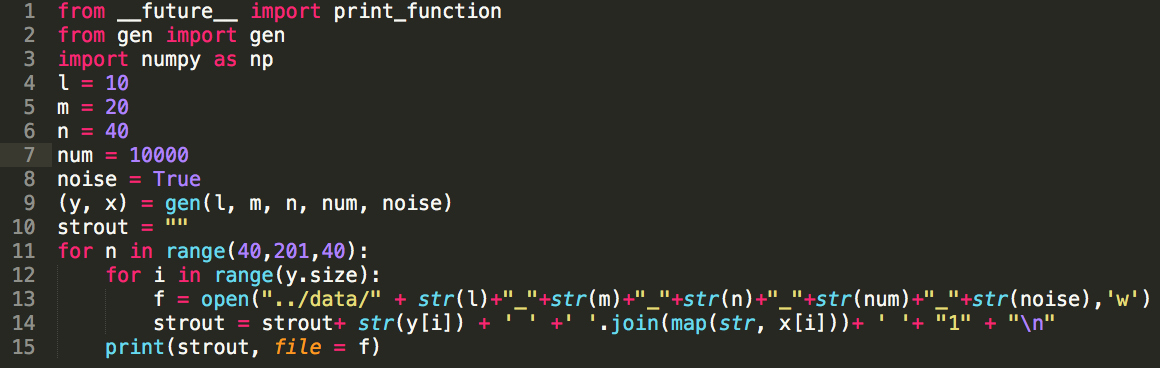
\includegraphics[width = 0.9\textwidth]{pythoncode4.png}
\item[(b)] Experiment
Use the parameter settings from Problem 3, $\eta$ = 0.25. Input l =10, m=20, n=40, noisy data as training data. Accumulate the loss after each round of training. For Hinge loss, sum up and record max(0, $1 - y(wx+\theta)$) in each round. On the other hand, sum up and record the mistakes made in each round. Then, plot the figure x axis means rounds and y axis means loss.\\
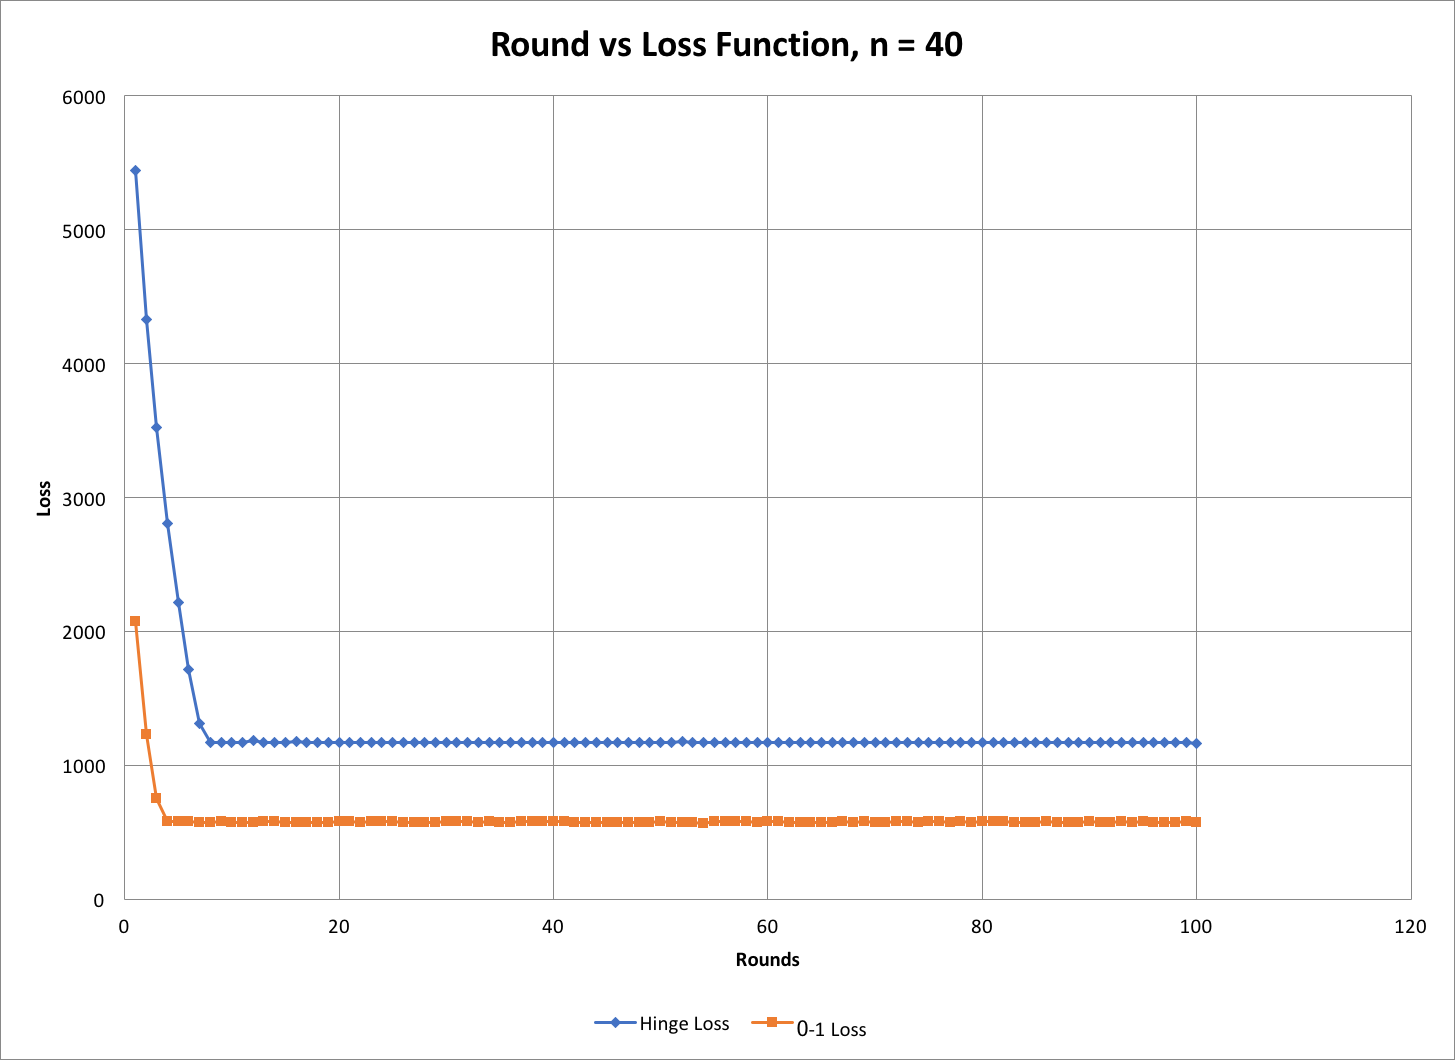
\includegraphics[width = 0.8\textwidth]{loss.png}\\
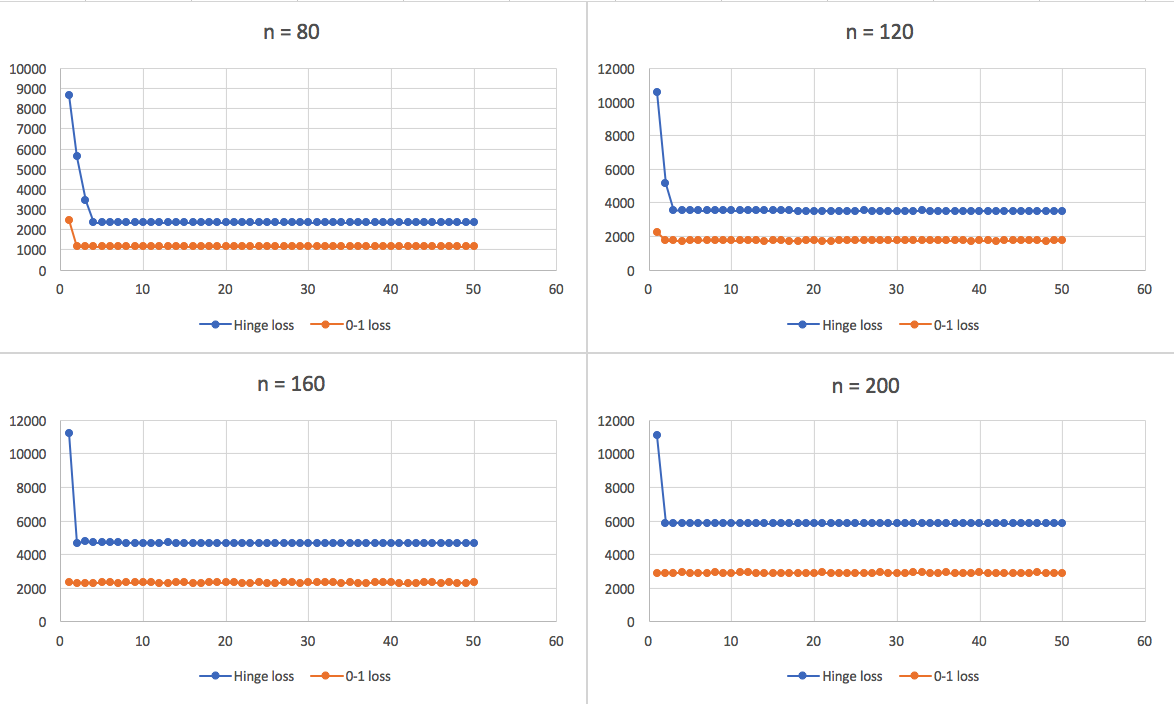
\includegraphics[width = 0.8\textwidth]{lossAll.png}\\
Observing the figure, we can conclude that after rounds of training process, AdaGrad algorithm converge. The Hinge loss and 0-1 loss are stable at last. It shows that after the algorithm converges the learning process, both 0-1 loss and Hinge loss still show the mistakes happen for training dataset. Comparing two losses, the Hinge loss is larger all the time. It is reasonable that even the classification is correct, $y(wx+\theta) > 0$, the example may still contribute to the Hinge error max(0, $1 - y(wx+\theta)$) if $1 - y(wx+\theta) > 0$. Besides, it can be observed that the higher n is the faster the algorithm converge. When n = 200, it converges almost at the first round.